\section{System}
\label{sec:system}

In this work we use the formulas from Kennedy's most recent definition of PSO~\cite{4223164}.
It can be easily extended to many versions of PSO.
This version of PSO includes a star topology, and a constricted position update rule. 
The constricted position update rule is
\begin{subequations}
\label{eq:pso_alg}
\begin{equation}
\label{eq:up_vel}
\begin{aligned}
v_{ij}(k+1) = &  \chi [ v_{ij}(k) 
 + \phi^{P} u^{P}_{ij}(k) (x^{P}_{ij}(k) - x_{ij}(k))\\
 & + \phi^{G} u^{G}_{ij}(k) ( x^{G}_{ij}(k) - x_{ij}(k)) ],
\end{aligned}
\end{equation}
\begin{equation}
\label{eq:up_pos}
x_{ij}(k+1) = x_{ij}(k) + v_{ij}(k+1).
\end{equation}
\end{subequations}
$ x_{ij}(k) $ represents the position of particle $ i $ in dimension $ j $ at time $ k $.
$ v_{ij}(k) $ similarly represents the velocity of particle $ i $ in dimension $ j $ also at time $ k $.
$ x^{G}_{ij}(k) $ and $ x^{P}_{ij}(k) $ are global (actually topology) and personal best positions observed by the swarm and the particle respectively. 
$ u^{G}_{ij}(k) $ and $ u^{P}_{ij}(k) $ are independent random values drawn from $ [0,1] $.
$ \chi \in ( 0, 1 ) $, $ \phi^{P} $ and $ \phi^{G} $ are algorithm parameters.

\begin{equation}
\label{eq:pb_up}
x^{P}(k) = \arg \max_{ x \in \{ x(k), x^{P}(k-1) \} } f(x)
\end{equation}
\begin{equation}
\label{eq:gb_up}
x^{G}(k) = \arg \max_{ x \in \{ x(k), x^{G}(k-1) \} } f(x)
\end{equation}

The organization of the swarm is implemented by the star topology.
When the position of a particle is chosen to be the global best, its personal best is updated as well.
In this case, $ x(k) = x^{P}(k) = x^{G}(k) $, which means this particle will not move till a new global best is found.
We could view this particle as a leader of this swarm.
The topology is given in Figure \ref{fig:leader_follower}.

\begin{figure}[tbph]
\centering
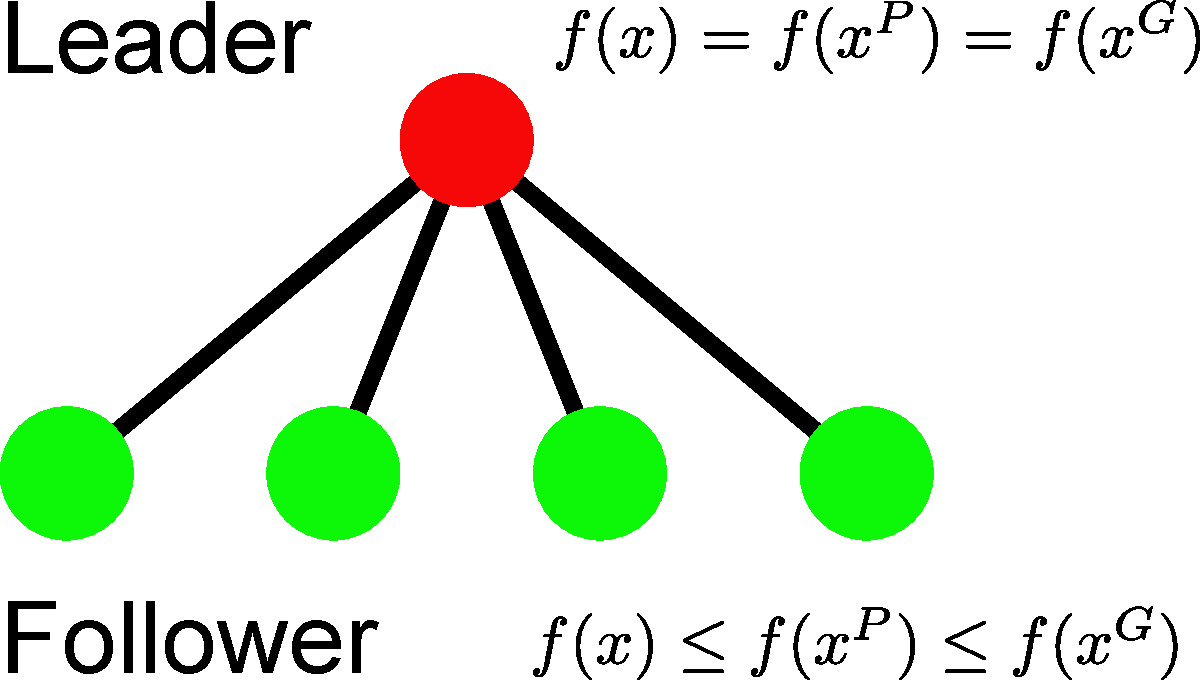
\includegraphics[width=0.5\linewidth]{./fig/leader_follower}
\caption{}
\label{fig:leader_follower}
\end{figure}

Thus, the star topology only provides a way of maintaining a leader competition among the particles.
Once a particle finds a new global best, it becomes the leader of the swarm.
The other particles are the followers, which are attracted to the leader by the impact of the global best.
By Property \ref{prop:unconverge_neq_gb}, we know that a particle will never stop moving if the personal best and the global best are inconsistent.
Thus, we can view the movements of the followers are sampling in the solution space to solve the inconsistency between its own personal best and the global best.
The input to each particle from the topology of the swarm is only the global best.

\subsection{A cascade model of a particle}

In this paper, we model the behavior of the PSO algorithm as a \emph{cascade system}.
%This enables analysis of PSO with stochastic factors preserved and without the stagnation assumption.
As shown in Figure \ref{fig:sys_flow}, this system is comprised of two components that form a cascade system structure.
These two components are the 
\emph{input update component} for the global best ($ x^{G}_{i}(k) $) and the personal best ($ x^{P}_{i}(k) $), and the 
\emph{position update component} for particle position ($ x_{i}(k+1) $), which depends on the inputs $ x^{G}_{i}(k) $ and $ x^{P}_{i}(k) $ as well as the last position $ x_{i}(k) $ and the swarm topology.

\begin{figure}
\centering
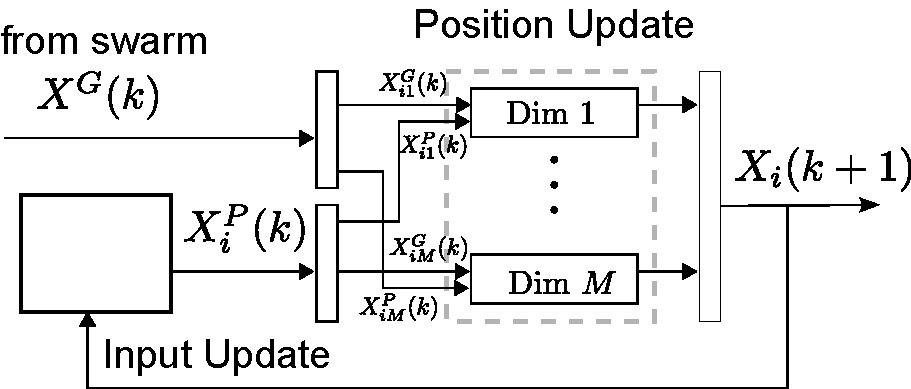
\includegraphics[width=0.85\linewidth]{./fig/sys_flow.pdf}
\caption{System structure of Particle.}
\label{fig:sys_flow}
\end{figure}

\begin{figure}
\centering
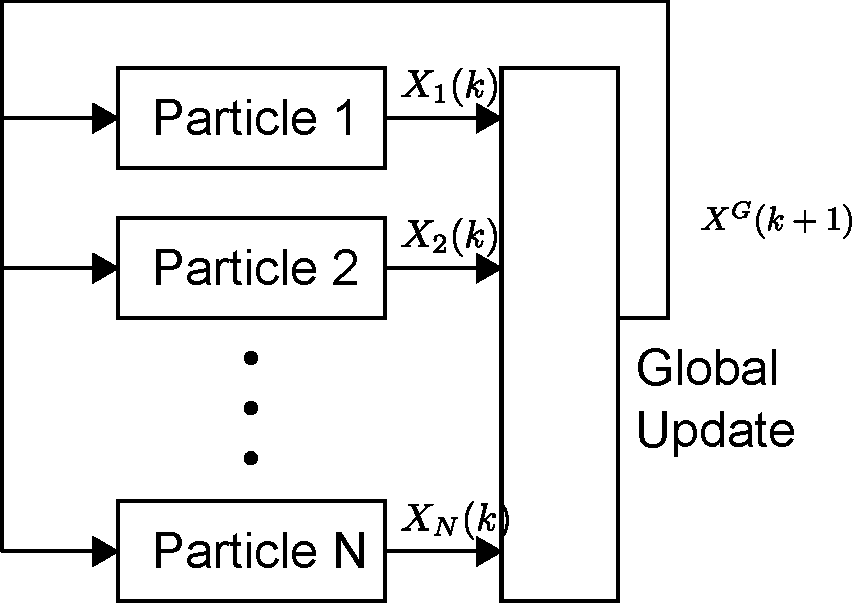
\includegraphics[width=0.6\linewidth]{./fig/pso_sys_flow.pdf}
\caption{System structure of Swarm}
\label{fig:pso_sys_flow}
\end{figure}

From Equation \eqref{eq:pso_alg}, we can write a linear form of the position update component in one dimension.
\begin{equation}
\label{eq:pso_up_linalg_simp}
X(k+1) = A(k) X(k) + B(k) U(k)
\end{equation}
with
$ A(k) = \begin{bmatrix}
\chi & - \chi \phi^{G} u^{G}(k) - \chi \phi^{P} u^{P}(k)
\\ 
\chi & 1 - \chi \phi^{G} u^{G}(k) - \chi \phi^{P} u^{P}(k)
\end{bmatrix} $
and
$ B(k) = \begin{bmatrix}
\chi \phi^{G} u^{G}(k) & \chi \phi^{P} u^{P}(k)
\\ 
\chi \phi^{G} u^{G}(k) & \chi \phi^{P} u^{P}(k)
\end{bmatrix} $.
The system state is $ X(k) = [ v(k), x(k) - x^{*} ]^{T} $, and the system input is $ U(k) = [ x^{G}(k) - x^{*} , x^{P}(k) - x^{*} ]^{T} $
\footnote{$ x^{*} $ means an equilibrium point to the system.
In PSO, it can be a local optimum, a global optimum, or an estimated optimum.
We use it as a reference point to check the bounds.}
With a new $ x(k+1) $ and the global best $ x^{G} $ from the topology of the swarm, the input update component will update the personal best $ x^{P}(k+1) $ and the global best $ x^{G}(k+1) $ that are fed into the position update component.

Because the position update works independently at each dimension.
When the solution space is multi-dimension, there is just a parallel-interconnection of the position update components of all the dimension.

The output of the input-update component is the input of the position-update component.
Take the same reference point $ x^{*} $, we can write the input-update component as 
\begin{equation}
\label{eq:pso_input_up}
U = g(V)
\end{equation}
with $ U = [ x^{P}(k) - x^{*} ]^{T} $ 
and $ V = [ x(k) - x^{*} ] $
from equation \eqref{eq:gb_up} and equation \eqref{eq:pb_up}. 
